% ---
% Capa
% ---
\imprimircapa
% ---

% ---
% Folha de rosto
% (o * indica que haverá a ficha catalográfica)
% ---
\imprimirfolhaderosto
% ---

% ---
% Ficha Catalografica em pdf e código
% 
% ---

%\begin{fichacatalografica}
%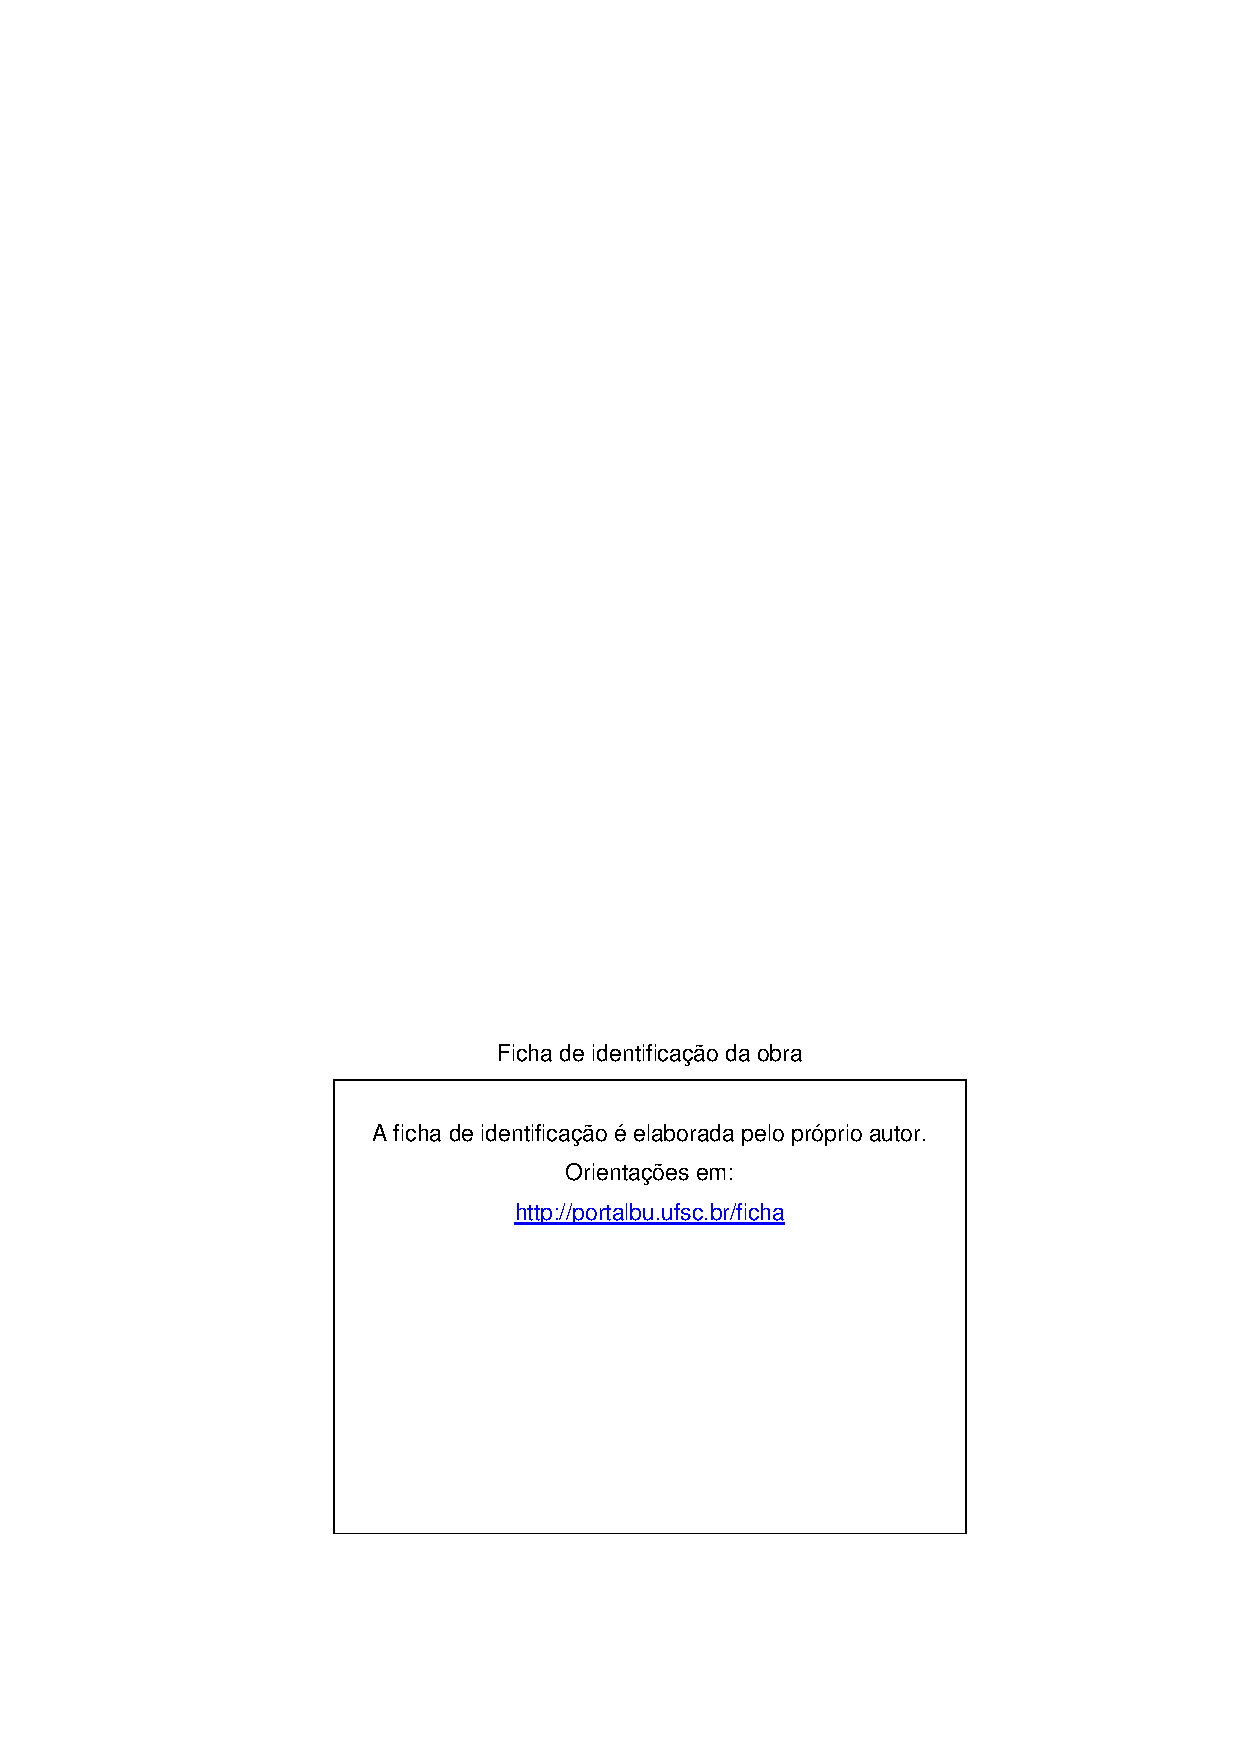
\includepdf{pre/Ficha_Catalografica.pdf}
%\end{fichacatalografica}

%Utilize este arquivo de ficha catalografica
%\begin{fichacatalografica}
\vspace*{12cm} % Posi��o vertical
%\hrule % Linha horizontal

\begin{center} % Minipage Centralizado
\small{\textbf{\cip}}
\framebox[120mm]{%Inicio da caixa
\begin{minipage}{105mm} % Largura [c]{12.5cm}
\begin{flushleft}
\codnome
\end{flushleft}
\MakeUppercase{\sobrenome},~\nome
%\tituloprincipal %\imprimirtitulo

\hspace{0.5cm} \tituloprincipal. / \nome~\sobrenome~ --~ %\imprimirautor
\imprimirlocal:~\sigla,~\imprimirano.\\

\hspace{0.5cm} \pageref{LastPage} p. : il.~color.~;~30 cm.\\

\hspace{0.5cm} \imprimirorientadorRotulo:~ \imprimirorientador.\\

\hspace{0.5cm} \imprimircoorientadorRotulo:~ \imprimircoorientador.\\

\hspace{0.5cm}
\parbox[t]{\textwidth}{\tcc~--~\imprimirinstituicao,~\campus~--~\imprimirprograma,~\imprimirano.}\\

\hspace{0.5cm}
1. \palavrachaveum.
2. \palavrachavedois.
3. \palavrachavetres.
4. \palavrachavequatro.
5. \palavrachavecinco.
I. \MakeUppercase{\sobrenomorient},~\nomorient~\sigorient..
II. \MakeUppercase{\sobrenomcoorient},~\nomcoorient~\sigcoorient..
%II. Universidade xxx.
%III. Faculdade de xxx.
III. T\'itulo.\\

%\hspace{7.75cm} \cdu\\
\begin{flushright}
    						\cdu
\end{flushright}%
%\hspace{8.75cm}
\end{minipage}
}%Fim caixa
\par
\vspace{0.1cm}
Ficha catalogr\'afica elaborada pelo bibliotec\'ario~\bibliotecario~\cbr
\par
Biblioteca Clarice Lispector
\par
\imprimirinstituicao
\par
\campus%Campus: An\'apolis

\end{center}

%\hrule
\end{fichacatalografica}%Retirando ficha catalografica

%----------------------------------------------


% ---
% Inserir folha de aprovação
% ---
%\includepdf[pages={1-2}]{arquivo.pdf}%utilizando duas paginas
%\includepdf[pages={5}, fitpaper=true]{Flauberth__Duarte_TCC.pdf}.
%\begin{folhadeaprovacao}
	\OnehalfSpacing
	\centering
	\imprimirautor\\%
	\vspace*{10pt}		
	\textbf{\imprimirtitulo}%
	\ifnotempty{\imprimirsubtitulo}{~\imprimirsubtitulo}\\%
	%		\vspace*{31.5pt}%3\baselineskip
	\vspace*{\baselineskip}
	%\begin{minipage}{\textwidth}
	% ~do~\imprimirprograma~do~\imprimircentro~da~\imprimirinstituicao~para~a~obtencao~do~t�tulo~de~\imprimirformacao.
	Este~\imprimirtipotrabalho~foi julgado adequado para obten\c{c}\~ao do T\'itulo de ''\imprimirformacao'' e aprovado em sua forma final pelo~\imprimirprograma. \\
		\vspace*{\baselineskip}
	\imprimirlocal, \imprimirdata. \\
	\vspace*{2\baselineskip}
	\assinatura{\OnehalfSpacing\imprimircoordenador \\ \imprimircoordenadorRotulo~do Curso}
	\vspace*{2\baselineskip}
	\textbf{Banca Examinadora:} \\
	\vspace*{\baselineskip}
	\assinatura{\OnehalfSpacing\imprimirorientador \\ \imprimirorientadorRotulo}
	%\end{minipage}%
%	\vspace*{\baselineskip}
%	\assinatura{Prof.\avaliadorinterno, \tituloavaliadorinterno\\ %Nao esta funcionando, ou seja, n�o faz altera�ao
%	Avaliador(\textsuperscript{o}) \\
%	Institui\c{c}\~ao xxxx}

%	\vspace*{\baselineskip}
%	\assinatura{Prof\textsuperscript{a}. \avaliadorexterno, Dr\textsuperscript{a}.\\%Nao esta funcionando, ou seja, n�o faz altera�ao
%	Avaliador(\textsuperscript{a}) \\
%	Institui\c{c}\~ao xxxx}


\end{folhadeaprovacao}
% ---%Retirando 


%---------------------------------------------------
\begin{folhaaprovacao}
    % As assinaturas dos avaliadores entram aqui (as outras já são automáticas)
    \vspace*{\baselineskip}
    \assinatura{Prof.\masculino~\avaliadorinterno, \tituloavaliadorinterno\\
    \avalinterno \\
    \entidadeinterna~(\siglainterno)}

    \vspace*{\baselineskip}
    \assinatura{Prof.\feminino~\avaliadorexterno, \tituloavaliadorexterno\\
    \avalexterno \\
    \entidadeexterna~(\siglaexterno)}
\end{folhaaprovacao}


%---------------------------------------------------

% ---
% Inserir folha de ata da seção pública de tcc
% ---
%\includepdf[pages={5}, fitpaper=true]{folhaDeAta.pdf}.
%% Altera o espa�amento para 1.5 apenas nesta p�gina
%\renewcommand{\baselinestretch}{1.5}\selectfont
%\linespread{0.90}%0.87
\linespread{0.87}\selectfont

%--------Cabe�alho do documento
\noindent\begin{minipage}[c][1.5cm][c]{3.5cm}
%\includegraphics[height=1.5cm]{./figuras/logoEvangelica.eps}

\includegraphics[width=1.5 \textwidth]{./outros/fig/IFGAnapolisHor2.png}
\end{minipage}\quad\quad\quad\qquad
\begin{minipage}{12cm}%10cm
\scriptsize\textbf{\ministerio}\\%\sc
\textbf{\secretaria}\\
\textbf{\instituto}\\
\textbf{\reitoria}\\
\end{minipage}
\vspace{1cm}
%---------------------------------------------------------------------------------------


\begin{center}
	\textbf{ATA N\textsuperscript{o} 20/\imprimirano}\\
	\footnotesize{\MakeUppercase{\textbf{Ata da sess\~ao p\'ublica de apresenta\c{c}\~ao do \imprimirtipotrabalho}}}
\end{center}
\vspace{1.0cm}
\noindent Aos~0\diaata~dias do m\^es de~\mesata~do ano de dois mil e vinte e cinco, \'as~\hinicial~horas, por meio de webconfer\^encia utilizando Google Meet, foi realizada a sess\~ao p\'ublica de apresenta\c{c}\~ao do \imprimirtipotrabalho~do Graduando~\textbf{\alunonome~\alunosobre}~(matr\'icula~\matricula) do~\imprimirprograma. A banca foi composta pelos seguintes membros:~\orientadora,~\membroum,~\membrodois, sob a presid\^encia da primeira. O \imprimirtipotrabalho~tem como t\'itulo ``\textbf{\titulo}'', sob orienta\c{c}\~ao da Prof\textsuperscript{a}~\orientadora. Ap\'os a apresenta\c{c}\~ao do \imprimirtipotrabalho, tendo sido o autor arguido pela Banca Examinadora, a nota obtida foi~\notanumerico~(\notaextenso).
\\
\\
\noindent Encerra-se a presente sess\~ao \'as~\hfinal~horas~e~\mfinal~minutos. Eu Prof\textsuperscript{a}.~\orientadora, dato e assino a presente ata que segue assinada por todos os membros da Banca e pelo graduando.
\vspace{1.0cm}
\small{
\begin{center}
\begin{tabular}{c}
\multicolumn{1}{c}{\asseletronica} \\ 
\multicolumn{1}{c}{Prof\textsuperscript{a}~\orientadora} \\ 
\multicolumn{1}{c}{} \\ 
\asseletronica \\ 
\multicolumn{1}{c}{Prof\textsuperscript{a}~\membroum~} \\ 
\multicolumn{1}{c}{~} \\ 
\asseletronica\\
%\includegraphics[width=0.30 \textwidth]{./outros/fig/AssDaniel.jpg} \\ %\hrulefill comando para linha
\multicolumn{1}{c}{Prof\textsuperscript{a}~\membrodois~} \\ 
\multicolumn{1}{c}{~} \\ 
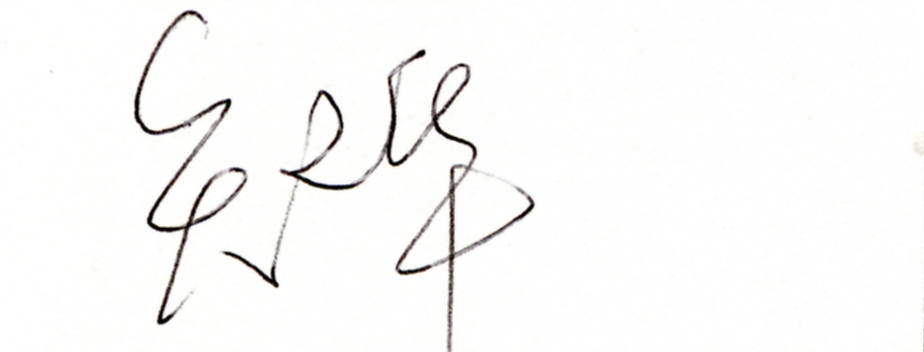
\includegraphics[width=0.25 \textwidth]{./outros/fig/minhaAssinatura2.png} \\
\multicolumn{1}{c}{\textbf{\alunonome~\alunosobre}} \\
\multicolumn{1}{c}{(Graduando)} \\
\multicolumn{1}{c}{~} \\ 
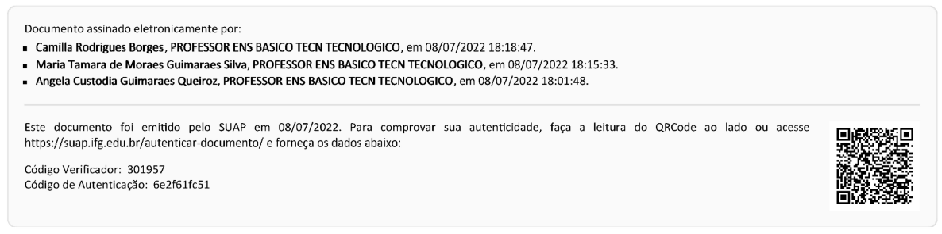
\includegraphics[width=0.97 \textwidth]{./outros/fig/QR_CODE_V2.pdf}
\\
\end{tabular}
\end{center}
}

% Restaura o espa�amento original para as pr�ximas p�ginas
%\renewcommand{\baselinestretch}{1.3}\selectfont
\linespread{1.3}\selectfont

\newpage%Retirando 

%---------------------------------------------------
\begin{comment}%Retire este comentario para aparecer a ata
%---------------------------------------------------
\begin{atareuniao}
\noindent Aos~\diaata~dias do mês de~\mesata~do ano de dois mil e vinte e cinco, às~\hinicial~horas, por meio de webconferência utilizando Google Meet, foi realizada a sessão pública de apresentação do \imprimirtipotrabalho~do Graduando~\textbf{\alunonome~\alunosobre}~(matrícula~\matricula) do~\imprimirprograma. A banca foi composta pelos seguintes membros:~\orientadora,~\avaliadorinterno,~\avaliadorexterno, sob a presidência da primeira. O \imprimirtipotrabalho~tem como título ``\textbf{\titulo}'', sob orientação da Prof\textsuperscript{a}~\orientadora. Após a apresentação do \imprimirtipotrabalho, tendo sido o autor arguido pela Banca Examinadora, a nota obtida foi~\notanumerico~(\notaextenso).

\vspace{0.5cm}
\noindent Encerra-se a presente sessão às~\hfinal~horas~e~\mfinal~minutos. Eu Prof\textsuperscript{a}.~\orientadora, dato e assino a presente ata que segue assinada por todos os membros da Banca e pelo graduando.

\vspace{0.1cm}
\vspace{-0.1cm} % Espaço negativo para "puxar" a tabela para cima
{\footnotesize 
\begin{center}
    % Ajusta o respiro global da tabela
    \renewcommand{\arraystretch}{0.8} 
    \begin{tabular}{c}
        \asseletronica \\[0.2cm] % <--- Adiciona 0.2cm de espaço APENAS aqui
        Prof\textsuperscript{a}~\orientadora \\[0.4cm] % Espaço maior entre pessoas
        
        \asseletronica \\[0.2cm]
        Prof\textsuperscript{a}~\avaliadorinterno \\[0.4cm] 
        
        \asseletronica \\[0.2cm]
        Prof\textsuperscript{a}~\avaliadorexterno \\[0.4cm] 
        
        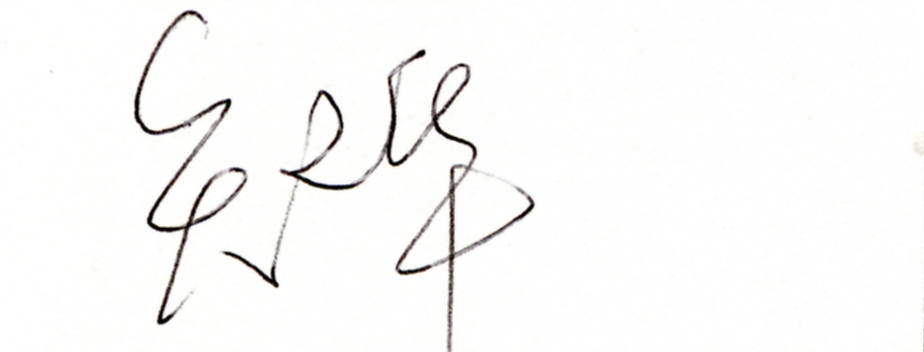
\includegraphics[width=0.20\textwidth]{./outros/fig/minhaAssinatura2.png} \\[0.1cm]
        \textbf{\alunonome~\alunosobre} \\
        (Graduando) \\[0.3cm] 
        
        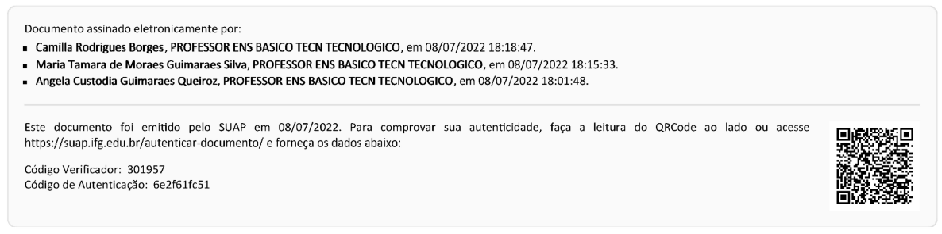
\includegraphics[width=0.79\textwidth]{./outros/fig/QR_CODE_V2.pdf}
    \end{tabular}
\end{center}
}
\end{atareuniao}
%---------------------------------------------------
\end{comment}
%---------------------------------------------------

% --------------------------------------------------
% Inserir folha de autorização para disponibilização
% --------------------------------------------------
%\linespread{0.87}\selectfont
%--------Cabe�alho do documento
\noindent\begin{minipage}[c][1.5cm][c]{3.5cm}

\includegraphics[width=1.5 \textwidth]{./outros/fig/IFGAnapolisHor2.png}
\end{minipage}\quad\quad\quad\qquad
\begin{minipage}{12cm}%10cm
\scriptsize\textbf{\ministerio}\\
\textbf{\secretaria}\\
\textbf{\instituto}\\
\textbf{\MakeTextUppercase{\campus}}\\
\textbf{\biblioteca}\\
\end{minipage}
%\vspace{-0.1cm}
\small{
\begin{center}
	\termo
\end{center}

\termodois

\noindent \textbf{Identifica\c{c}\~ao de Produ\c{c}\~ao T\'ecnico-Cient\'ifica}

\begin{tabular}{lllll}
\lbrack ~~\rbrack & Tese &  & \lbrack ~~\rbrack & Artigo Cient\'ifico \\ 
\lbrack ~~\rbrack & Disserta\c{c}\~ao &  & \lbrack ~~\rbrack & Cap\'itulo de Livro \\ 
\lbrack ~~\rbrack & Monografia -- Especializa\c{c}\~ao &  & \lbrack ~~\rbrack & Livro \\ 
\lbrack X\rbrack & TCC -- Gradua\c{c}\~ao &  & \lbrack ~~\rbrack & Trabalho Apresentado em Evento \\ 
\lbrack ~~\rbrack & Produto T\'ecnico e Educacional -- Tipo: & \multicolumn{3}{l}{\hrulefill} \\ 
\end{tabular}

\quad

\noindent Nome Completo do Autor:~\textbf{\alunonome~\alunosobre}

\noindent Matr\'icula:~\textbf{\matricula}

\noindent T\'ituto do Trabalho:~\textbf{\tituloprincipal}

\noindent \textbf{Autoriza\c{c}\~ao -- Marque uma das op\c{c}\~oes}

\begin{enumerate}
	\item (X) Autorizo disponibilizar meu trabalho no Reposit\'orio Digital do IFG (acesso aberto);
	\item (~) Autorizo disponibilizar meu trabalho no Reposit\'orio Digital do IFG somente ap\'os a data 20/10/20 (Embargo);
	\item (~) N\~ao autorizo disponibilizar meu trabalho no Reposit\'orio Digital do IFG (acesso restrito)
\end{enumerate}

\noindent Ao indicar a op\c{c}\~ao \textbf{2 ou 3}, marque a justificativa:
\begin{description}
	\item[(~~)] O documento est\'a sujeito a registro de patente.
	\item[(~~)] O documento pode vir a ser publicado como livro, cap\'itulo de livro ou artigo.
	\item[(~~)] Outra justificativa: \hrulefill
\end{description}

\begin{center}
	\textbf{\declaracao}
\end{center}

\noindent O(A) referido(a) autor(a) declara que:

\textbf{(i)}~o documento \'e seu trabalho original, det\'em os direitos autorais de produ\c{c}\~ao t\'ecnico-cient\'ifica e n\~ao infringe os direitos de qualquer outro pessoa ou entidade;

\textbf{(ii)}~\termotres

\textbf{(iii)}~cumpriu quaisquer obriga\c{c}\~oes exigidas por contrato ou acordo, caso o documento entregue seja baseado em trabalho finaciado ou apoiado por outra institui\c{c}\~ao que n\~ao o \entidade.

%\todaydia
\begin{flushright}
An\'apolis, {\diaata~de~\mesata}~de~{\todayano}
\end{flushright}

\begin{center}
\begin{tabular}{c}
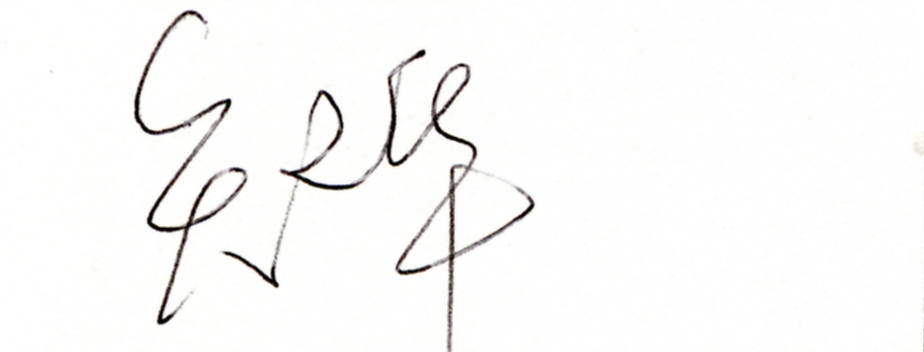
\includegraphics[width=0.19 \textwidth]{./outros/fig/minhaAssinatura2.png} \\ 
\multicolumn{1}{c}{~\alunonome \alunosobre} \\ 
%\multicolumn{1}{c}{\hrulefill} \\ 
\end{tabular}
\end{center}
}%Fim \small

\linespread{1.3}\selectfont
%Retirando 
%\includepdf[pages={5}, fitpaper=true]{folhaTermo.pdf}.
%---------------------------------------------------
\begin{comment}% Descomente para aparecer O Termo de Autorização da biblioteca

\linespread{0.87}\selectfont
%--------Cabeçalho do documento
\noindent\begin{minipage}[c][1.5cm][c]{3.5cm}

\includegraphics[width=1.5 \textwidth]{./outros/fig/IFGAnapolisHor2.png}
\end{minipage}\quad\quad\quad\qquad
\begin{minipage}{12cm}%10cm
\scriptsize\textbf{\ministerio}\\
\textbf{\secretaria}\\
\textbf{\instituto}\\
\textbf{\MakeTextUppercase{\campus}}\\
\textbf{\biblioteca}\\
\end{minipage}
%\vspace{-0.1cm}
\small{
\begin{center}
	\termo
\end{center}

\termodois

\noindent \textbf{Identifica\c{c}\~ao de Produ\c{c}\~ao T\'ecnico-Cient\'ifica}

\begin{tabular}{lllll}
\lbrack ~~\rbrack & Tese &  & \lbrack ~~\rbrack & Artigo Cient\'ifico \\ 
\lbrack ~~\rbrack & Disserta\c{c}\~ao &  & \lbrack ~~\rbrack & Cap\'itulo de Livro \\ 
\lbrack ~~\rbrack & Monografia -- Especializa\c{c}\~ao &  & \lbrack ~~\rbrack & Livro \\ 
\lbrack X\rbrack & TCC -- Gradua\c{c}\~ao &  & \lbrack ~~\rbrack & Trabalho Apresentado em Evento \\ 
\lbrack ~~\rbrack & Produto T\'ecnico e Educacional -- Tipo: & \multicolumn{3}{l}{\hrulefill} \\ 
\end{tabular}

\quad

\noindent Nome Completo do Autor:~\textbf{\alunonome~\alunosobre}

\noindent Matr\'icula:~\textbf{\matricula}

\noindent T\'ituto do Trabalho:~\textbf{\tituloprincipal}

\noindent \textbf{Autoriza\c{c}\~ao -- Marque uma das op\c{c}\~oes}

\begin{enumerate}
	\item (X) Autorizo disponibilizar meu trabalho no Reposit\'orio Digital do IFG (acesso aberto);
	\item (~) Autorizo disponibilizar meu trabalho no Reposit\'orio Digital do IFG somente ap\'os a data 20/10/20 (Embargo);
	\item (~) N\~ao autorizo disponibilizar meu trabalho no Reposit\'orio Digital do IFG (acesso restrito)
\end{enumerate}

\noindent Ao indicar a op\c{c}\~ao \textbf{2 ou 3}, marque a justificativa:
\begin{description}
	\item[(~~)] O documento est\'a sujeito a registro de patente.
	\item[(~~)] O documento pode vir a ser publicado como livro, cap\'itulo de livro ou artigo.
	\item[(~~)] Outra justificativa: \hrulefill
\end{description}

\begin{center}
	\textbf{\declaracao}
\end{center}

\noindent O(A) referido(a) autor(a) declara que:

\textbf{(i)}~o documento \'e seu trabalho original, det\'em os direitos autorais de produ\c{c}\~ao t\'ecnico-cient\'ifica e n\~ao infringe os direitos de qualquer outro pessoa ou entidade;

\textbf{(ii)}~\termotres

\textbf{(iii)}~cumpriu quaisquer obriga\c{c}\~oes exigidas por contrato ou acordo, caso o documento entregue seja baseado em trabalho finaciado ou apoiado por outra institui\c{c}\~ao que n\~ao o \entidade.

%\todaydia
\begin{flushright}
An\'apolis, {\diaata~de~\mesata}~de~{\todayano}
\end{flushright}

\begin{center}
\begin{tabular}{c}
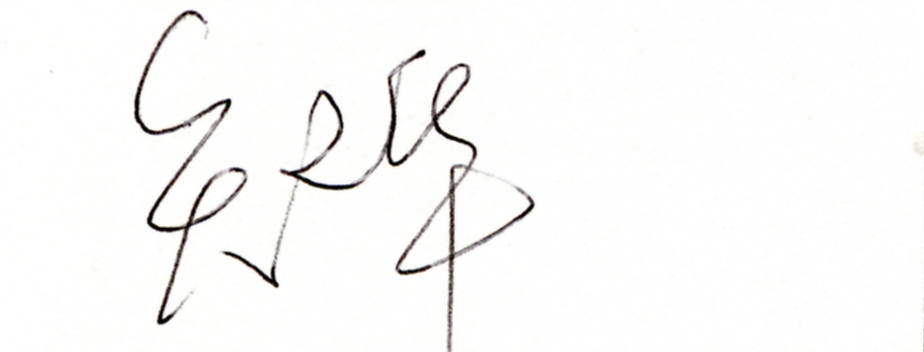
\includegraphics[width=0.19 \textwidth]{./outros/fig/minhaAssinatura2.png} \\ 
\multicolumn{1}{c}{~\alunonome \alunosobre} \\ 
%\multicolumn{1}{c}{\hrulefill} \\ 
\end{tabular}
\end{center}
}%Fim \small

\linespread{1.3}\selectfont

\end{comment}
%---------------------------------------------------


% ---
% Dedicatória
% ---
%\begin{dedicatoria}
%	\vspace*{\fill}
%	\noindent
%	\begin{adjustwidth*}{}{5.5cm}     
%		Este trabalho é dedicado aos meus colegas de %classe e aos meus queridos pais.
%	\end{adjustwidth*}
%\end{dedicatoria}
% ---

% ---
% Agradecimentos
% ---
%\begin{agradecimentos}
%	Inserir os agradecimentos aos colaboradores à %execução do trabalho. 
%\end{agradecimentos}
% ---

% ---
% Epígrafe
% ---
\begin{epigrafe}
    \null\vfill % Cria o ponto no topo e empurra o conteúdo para baixo
		\vspace{3cm}
    \begin{flushright}
        \textit{Se você for receptivo e humilde, a matemática o conduzirá pela mão. Repetidas vezes, quando estive perdido sem saber como prosseguir, bastou-me esperar até sentir que a matemática me guiava pela mão. Ela me conduziu por um caminho inesperado, um caminho onde novas perspectivas se abrem, um caminho que leva a um território novo, onde é possível estabelecer uma base de operações, a partir da qual se pode observar os arredores e planejar o progresso futuro.} \\
        \vspace{0.3cm}
        (Paul Dirac)
    \end{flushright}
    \vspace*{0.5cm} % Garante uma margem mínima do fim da folha (ajuste se quiser mais baixo)
\end{epigrafe}



% ---

% ---
% RESUMOS
% ---

% resumo em português
\setlength{\absparsep}{18pt} % ajusta o espaçamento dos parágrafos do resumo
\begin{resumo}
\SingleSpacing
%Os resultados revelam que não existe uma técnica universalmente superior: o RLM-\textit{subagging} apresentou melhor desempenho para Mn e Ni, o RLM-\textit{bagging} mostrou-se superior para Fe, enquanto a RLM clássica demonstrou desempenho superior para Mo e Cr. O comportamento diferenciado entre os analitos é atribuído à complexidade espectral de cada elemento: o Fe, por apresentar maior densidade de linhas espectrais com potencial de autoabsorção e sobreposições com outros elementos da matriz, beneficia-se da agregação de múltiplos modelos. Em contrapartida, Mn, Mo, Cr e Ni têm sua relação espectral-concentração suficientemente capturada pela RLM clássica ou pelo RLM-\textit{subagging}, sem ganho adicional com o RLM-\textit{bagging}. Todos os modelos apresentaram R$^2$ superior a 0,9815, evidenciando elevada capacidade preditiva. Quanto à eficiência computacional, o RLM-\textit{subagging} mostrou-se em média 3,0 vezes mais rápido que o RLM-\textit{bagging}, configurando-se como alternativa equilibrada entre precisão e eficiência em aplicações quimiométricas sujeitas a restrições temporais.

A calibração multivariada é essencial para determinar a composição elementar de aço-ligas a partir de dados espectrométricos. Este trabalho investigou, em caráter exploratório, a aplicação das técnicas de reamostragem \textit{bootstrap}, \textit{bagging} e \textit{subagging} incorporadas à Regressão Linear Múltipla (RLM) para a estimativa quantitativa dos elementos Manganês (Mn), Molibdênio (Mo), Cromo (Cr), Níquel (Ni) e Ferro (Fe). Paralelamente, conduziu-se a modernização de um sistema legado monolítico em Java \textit{Desktop} para uma aplicação \textit{Web} em Python e Streamlit, adotando arquitetura desacoplada em três módulos de responsabilidade única. A validação do sistema reescrito e a fidelidade a lógica matemática original foram asseguradas por uma suíte de 92 testes automatizados desenvolvida com \texttt{pytest}, englobando 21 testes unitários, 60 testes de caixa-preta baseados nos arquivos do sistema legado e 11 testes de carga e estresse com matrizes de alta dimensão. Os resultados experimentais demonstraram que a eficiência das técnicas de \textit{ensemble} varia conforme o analito: a RLM clássica obteve menor \textit{Root-Mean-Square Error of Prediction} (RMSEP) para o Molibdênio e o Cromo; o RLM-\textit{bagging} obteve menor erro para o Ferro; e o RLM-\textit{subagging} apresentou melhor desempenho para o Manganês e o Níquel (neste último, com desempenho numericamente equivalente ao da RLM clássica, com diferença de 0,25\% no (RMSEP). Em termos de eficiência computacional, o RLM-\textit{subagging} reduziu o tempo de processamento em relação ao RLM-\textit{bagging} em quatro dos cinco analitos. A suíte de testes confirmou a equivalência numérica estrita para os métodos determinísticos e a estabilidade da aplicação sob exigência computacional elevada, comprovando a viabilidade da modernização arquitetural sem perda de acurácia científica.

\textbf{Palavras-chave}: \palavrachaveum. \palavrachavedois. \palavrachavetres. \palavrachavequatro. \palavrachavecinco.
\end{resumo}

% resumo em inglês
\begin{resumo}[Abstract]
\SingleSpacing
\begin{otherlanguage*}{english}
%---------------------------------------------------
%The results reveal that no universally superior technique exists: RLM-\textit{subagging} achieved the best performance for Mn and Ni, RLM-\textit{bagging} proved superior for Fe, while classical MLR demonstrated superior performance for Mo and Cr. The differentiated behavior among analytes is attributed to the spectral complexity of each element: Fe, due to its higher density of spectral lines with self-absorption potential and overlaps with other matrix elements, benefits from the aggregation of multiple models. In contrast, Mn, Mo, Cr and Ni have their spectral-concentration relationship sufficiently captured by classical MLR or MLR-\textit{subagging}, with no additional gain from MLR-\textit{bagging}. All models presented R$^2$ values above 0.9815, evidencing high predictive capacity. Regarding computational efficiency, MLR-\textit{subagging} proved on average 3.0 times faster than MLR-\textit{bagging}, establishing itself as a balanced alternative between accuracy and efficiency in chemometric applications subject to time constraints.
%------------------------

Multivariate calibration is essential for determining the elemental composition of alloy steels from spectrometric data. This study explored the application of bootstrap resampling, bagging, and subagging techniques incorporated into Multiple Linear Regression (MLR) for the quantitative estimation of Manganese (Mn), Molybdenum (Mo), Chromium (Cr), Nickel (Ni), and Iron (Fe). Concurrently, a legacy monolithic Java Desktop system was modernized into a Python and Streamlit Web application, adopting a decoupled architecture structured into three single-responsibility modules. The validation of the rewritten system and its fidelity to the original algorithmic core were ensured by a suite of 92 automated tests developed with pytest, encompassing 21 unit tests, 60 black-box tests based on legacy system outputs, and 11 load and stress tests with high-dimensional matrices. Experimental results demonstrated that the efficiency of ensemble techniques varies depending on the analyte: classical MLR achieved a lower Root-Mean-Square Error of Prediction (RMSEP) for Molybdenum and Chromium; MLR-bagging yielded the lowest error for Iron; and MLR-subagging exhibited superior performance for Manganese and Nickel (in the latter, with performance numerically equivalent to classical MLR, showing a 0.25\% difference in RMSEP). In terms of computational efficiency, MLR-subagging reduced processing time compared to MLR-bagging across four of the five analytes. The test suite confirmed strict numerical equivalence for deterministic methods and application stability under high computational demand, proving the feasibility of architectural modernization without loss of scientific accuracy.%


%------------------------

\textbf{Keywords}: Resampling. Multivariate Calibration. Bagging. Subagging. Chemometrics.
\end{otherlanguage*}
\end{resumo}

%% resumo em francês 
%\begin{resumo}[Résumé]
% \begin{otherlanguage*}{french}
%    Il s'agit d'un résumé en français.
% 
%   \textbf{Mots-clés}: latex. abntex. publication de textes.
% \end{otherlanguage*}
%\end{resumo}
%
%% resumo em espanhol
%\begin{resumo}[Resumen]
% \begin{otherlanguage*}{spanish}
%   Este es el resumen en español.
%  
%   \textbf{Palabras clave}: latex. abntex. publicación de textos.
% \end{otherlanguage*}
%\end{resumo}
%% ---

{%hidelinks
	\hypersetup{hidelinks}
	% ---
	% inserir lista de ilustrações
	% ---
	\pdfbookmark[0]{\listfigurename}{lof}
	\listoffigures* %Retirado
	\cleardoublepage
	% ---
	
	% ---
	% inserir lista de quadros
	% ---
	\pdfbookmark[0]{\listofquadrosname}{loq}
	\listofquadros* %Retirado
	\cleardoublepage
	% ---
	
	% ---
	% inserir lista de tabelas
	% ---
	\pdfbookmark[0]{\listtablename}{lot}
	\listoftables* %Retirando
	\cleardoublepage
	% ---
	
	% ---
	% inserir lista de abreviaturas e siglas (devem ser declarados no preambulo)
	% ---

\imprimirlistadesiglas %Retirando
%\cleardoublepage
	% ---
	
	% ---
	% inserir lista de símbolos (devem ser declarados no preambulo)
	% ---
\imprimirlistadesimbolos %Retirando
%\cleardoublepage
	% ---
	
	% ---
	% inserir o sumario
	% ---
	\pdfbookmark[0]{\contentsname}{toc}
	\tableofcontents*
	\cleardoublepage
	
}%hidelinks
% ---
